%%%%%%%%%%%%%%%%%%%%%%%%%%%%%%%%%%%%%%%%%%%%%%%%%%%%%%%%%%%%%%%%%%%%%%
% How to use writeLaTeX: 
%
% You edit the source code here on the left, and the preview on the
% right shows you the result within a few seconds.
%
% Bookmark this page and share the URL with your co-authors. They can
% edit at the same time!
%
% You can upload figures, bibliographies, custom classes and
% styles using the files menu.
%
%%%%%%%%%%%%%%%%%%%%%%%%%%%%%%%%%%%%%%%%%%%%%%%%%%%%%%%%%%%%%%%%%%%%%%

\documentclass[12pt]{article}
\usepackage{sbc-template}

\usepackage{graphicx,url,xcolor,enumerate}
\usepackage{placeins}
\usepackage{float}

\usepackage[brazil]{babel}   
\usepackage{titlesec}
\usepackage[utf8]{inputenc}  

\titlespacing{\section}
{0pt}{5.5ex plus 1ex minus .2ex}{4.3ex plus .2ex}
\titlespacing{\subsection}
{0pt}{5.5ex plus 1ex minus .2ex}{4.3ex plus .2ex}

\sloppy

\title{Estudo de caracterização de aplicações desktop de repositórios do Github por meio de Inteligência Artificial}

\author{Guilherme Gabriel S. Pereira, Henrique P. F. Monteiro, Lucas Ângelo O. M. Rocha, 
\\ Victor B. G. Campos, Vinícius M. C. e Oliveira, Professor Felipe Augusto Lima Reis, 
\\ Professor José Laerte Pires Xavier Junior }


\address{Unidade Praça da Liberdade -- Pontifícia Universidade Católica de Minas Gerais
  (PucMinas)\\
  Belo Horizonte -- MG -- Brazil
\nextinstitute
  Departamento de Engenharia de Software e Sistemas de Informação -- PucMinas\\
  Belo Horizonte, MG.
\email{\{ggspereira,laomrocha,henrique.forte,vinicius.marini,vbgcampos\}@sga.pucminas.br}
\email{\{felipe.reis.4529302,laertexavier\}@pucminas.br}
}

\begin{document} 

\maketitle 

\begin{abstract}
  
\end{abstract}
     
\begin{resumo} 
  
\end{resumo}


\section{Introdução} \label{introducao}

Um desafio atual para empresas de software e desenvolvedores independentes é escolher entre plataformas web, mobile e desktop para suas aplicações, visando alcançar com mais eficácia seus usuários~\cite{9463138}. O sucesso de um novo produto de software está relacionado com sua forma disponibilização ao público, consequentemente ligado a qual plataforma ele está disponível. Sendo válido ressaltar que um mesmo software não está restrito a apenas uma plataforma, mas é recomendável uma análise prévia antes de disponibilizar um sistema em mais de uma plataforma, porque será mais caro e terá mais custos de manutenção~\cite{Eke2019}. Diante disso, durante essa análise, há o problema de definir se é conveniente implementar uma solução do software para a plataforma desktop, sendo necessário saber os objetivos mais populares e corriqueiros das aplicações desenvolvidas para desktop na atualidade e se são compatíveis com os objetivos da aplicação em análise.

O problema a ser solucionado nesta pesquisa, é a carência de um estudo específico que busque analisar e classificar os objetivos mais comuns de aplicações desktop hodiernamente. A partir desta pesquisa, tem-se um estudo no qual é possível compreender quais são os domínios mais recorrentes e as popularidades destes domínios no contexto de aplicações desenvolvidas para a plataforma desktop. Aplicações desktop referem-se aos sistemas desenvolvidos para a plataforma desktop e seus domínios podem ser definidos como os adjetivos definidos pelos objetivos que a aplicação se propõe, como, por exemplo, aplicações desktop que buscam detectar e eliminar vírus, são definidas no domínio antivírus.

A motivação na qual levou desenvolver-se esta pesquisa é compreender melhor o cenário atual de aplicações desktop após o aumento no uso de aplicações mobile, fortemente influenciado pela pandemia da COVID-19~\cite{KATSUMATA2022100168}. Busca-se adquirir um maior conhecimento sobre aplicações desktop, seus domínio e popularidade das aplicações da plataforma desktop. 

Assim, o trabalho justifica-se, porque desenvolvedores, gestores de novos projetos e analistas de sistemas podem analisar estas informações e decidir com mais confiança se compensa desenvolver seu produto para a plataforma desktop, diminuindo as chances de iniciar o desenvolvimento de uma aplicação desktop para um domínio desktop que já esteja em declínio de uso e popularidade. Desta forma, este estudo auxilia os responsáveis por produtos de software a implementar aplicações para os domínios populares no contexto desktop, por meio da caracterização dos principais domínios de aplicações desktop da atualidade.

Este trabalho tem como objetivo geral explorar e caracterizar aplicações desktop e seus respectivos domínios, com relação às suas métricas por domínios e popularidade, no contexto dos repositórios do Github que possuem dependências de aplicações desktop das linguagens C\# e JavaScript. Desta forma, para alcançar resultados, foram delimitados objetivos específicos, por meio das seguintes três questões de pesquisa e suas respectivas métricas:

\begin{enumerate}
  \item[QP.1] Para as aplicações desktop que ainda são mantidas, qual o domínio que elas se encontram atualmente?
    \begin{enumerate}
        \item[M.1] Proporção de repositórios que possuem descrições e domínios contra que não possuem descrições ou domínios;
        \item[M.2] Percentual da quantidade de repositórios desktops para cada domínio.
    \end{enumerate}
  \item[QP.2] A quantidade de aplicações desktop vem diminuindo ao longo da última década?
    \begin{enumerate}
        \item[M.3] Média de repositórios de aplicações desktops criados por ano para cada domínio;
        \item[M.4] Média de repositórios de aplicações desktops criados por ano.
    \end{enumerate}
  \item[QP.3] Aplicações desktop tem engajamento da comunidade?
    \begin{enumerate}
        \item[M.5] Percentual de \textit{pull requests merged} em relação aos não \textit{merged} dos repositórios desktop por ano;
        \item[M.6] Percentual de \textit{issues} fechadas em relação a não fechadas em repositórios de aplicações desktops por ano.
    \end{enumerate}
\end{enumerate}

A organização do conteúdo a seguir deste trabalho se define da seguinte forma: a Seção \ref{trabalhosrelacionados} são caracterizados os trabalhos relacionados; já a Seção \ref{metodologia} aborda as técnicas utilizadas para responder às questões formuladas através do objetivo; na Seção \ref{resultados} são apresentados os resultados encontrados para responder às questões da pesquisa.

\section{Trabalhos Relacionados} \label{trabalhosrelacionados}

Nesta seção são abordados os artigos já encontrados na literatura, usados para guiar a pesquisa do presente trabalho.

Sobre a caracterização de aplicações, a pesquisa realizada por Robert Lokaiczyk ~\cite{4561878} descreve como objetivo investigar a viabilidade do uso de técnicas não supervisionadas para a classificação taxonômica de aplicações Desktop, ou seja, o domínio de determinada aplicação, com base nos \textit{logs} gerados pelas aplicações. Para tal, foram utilizados dois métodos diferentes: análise de co-ocorrência e análise de cluster. Foi concluído que ambas abordagens produziam um resultado com acurácia satisfatória. O método de classificação se difere do apresentado no presente trabalho, pois este não necessita da execução do sistema para efetuar a classificação.

Se tratando das tecnologias usadas em aplicações desktop, o estudo realizado por Hazar, Zinah e Toman ~\cite{toman2019depth} comparou os principais \textit{frameworks} de \textit{software} para desenvolvimento dessas aplicações usando tecnologias da web, Electron e NW.js, por um estudo de caso e uma análise de conteúdo, comparando diversas características entre os \textit{frameworks}, como arquitetura, ferramentas para construir a interface com o usuário, e facilidade de integração com sistemas. Levantando todos os prós e contras dos \textit{frameworks}, o Electron se mostrou como o mais adequado, principalmente no que diz respeito à integração de sistemas, a interface com o usuário, sistema de arquivos e funcionalidades multimídia. Esse artigo contribui para a escolha do Electron como tecnologia a ser pesquisada no presente trabalho.

Utilizando de um estudo de caso, Katsumata ~\cite{KATSUMATA2022100168} realiza uma análise das mudanças do uso de dispositivos móveis durante a pandemia do COVID-19. Mais especificamente, o estudo coletou dados de utilização dos dispositivos no Japão, analisando os períodos do primeiro e segundo pico do coronavírus. O objetivo deste artigo foi analisar as mudanças no uso de dispositivos móveis durante a crise do COVID-19. Os autores concluem que o uso de dispositivos móveis aumentou significativamente durante a pandemia, com as pessoas se voltando para eles para se manter conectadas e informadas. Considerando esse aumento, essa pesquisa contribui para um dos questionamentos proposto no presente trabalho, de que estaria havendo uma diminuição das aplicações desktop, no geral.

Em relação às métricas escolhidas, o estudo de Yamamoto~\cite{9282287} visa entender quais métricas devem ser usadas para buscar repositórios em pesquisas científicas para diversos casos. O trabalho faz a análise de diversos repositórios, alterando os critérios de busca. Alguns destaques encontrados na pesquisa são o uso de número de contribuidores do repositório e busca por dependências. Neste contexto, o artigo foi utilizado para discussão de qual os critérios deveriam ser usados na escolha dos repositórios a serem analisados. No caso, o número de estrelas foi um dos apontados como critério de popularidade.

Sobre o método classificatório, o trabalho de Radford ~\cite{radford2018improving} apresenta o GPT (\textit{Generative Pre-Training}), o método usado para treinar modelos de linguagem. O método se baseia em uma etapa de pré-treinamento não supervisionado, seguido de uma etapa de ajuste fino, ou afinação. Os testes demonstraram que este \textit{framework} consegue produzir modelos capazes de executar diversas tarefas de processamento de linguagem natural, como responder a perguntas, tarefas de similaridade semântica e classificação. O modelo descrito é usado no presente trabalho, mais especificamente, para a tarefa de classificação de domínios dos repositórios.

\section{Metodologia} \label{metodologia}

\subsection{Visão Geral}

Esta pesquisa tem como escopo, buscar projetos \textit{open-source} no Github que se enquadram na categoria de aplicações desktop e validar se seus domínios ainda possuem popularidade. Para esse propósito foram coletadas as descrições, \textit{pull requests} e \textit{issues} de repositórios mais populares das linguagens C\# e Javascript, que possuíam alguma dependência \textit{desktop}. 

O processo de análise está dividido em cinco etapas, ilustrado na Figura \ref{fig:Metodologia} e explicitado a seguir: 1. Coleta de repositórios; 2. Recolhimento de \textit{issues} e \textit{pull requests}; 3. Análise de domínio utilizando inteligência artificial; 4. Filtragem manual de domínios; 5. Reavaliação de repositórios com domínios definidos.

Para a realização das etapas, com exceção da quarta etapa, foram criados \textit{scripts} na linguagem Python para realizar a coleta e processamento e, todas as informações obtidas foram salvas em um banco de dados relacional local.

\begin{figure}[H]
    \centering
    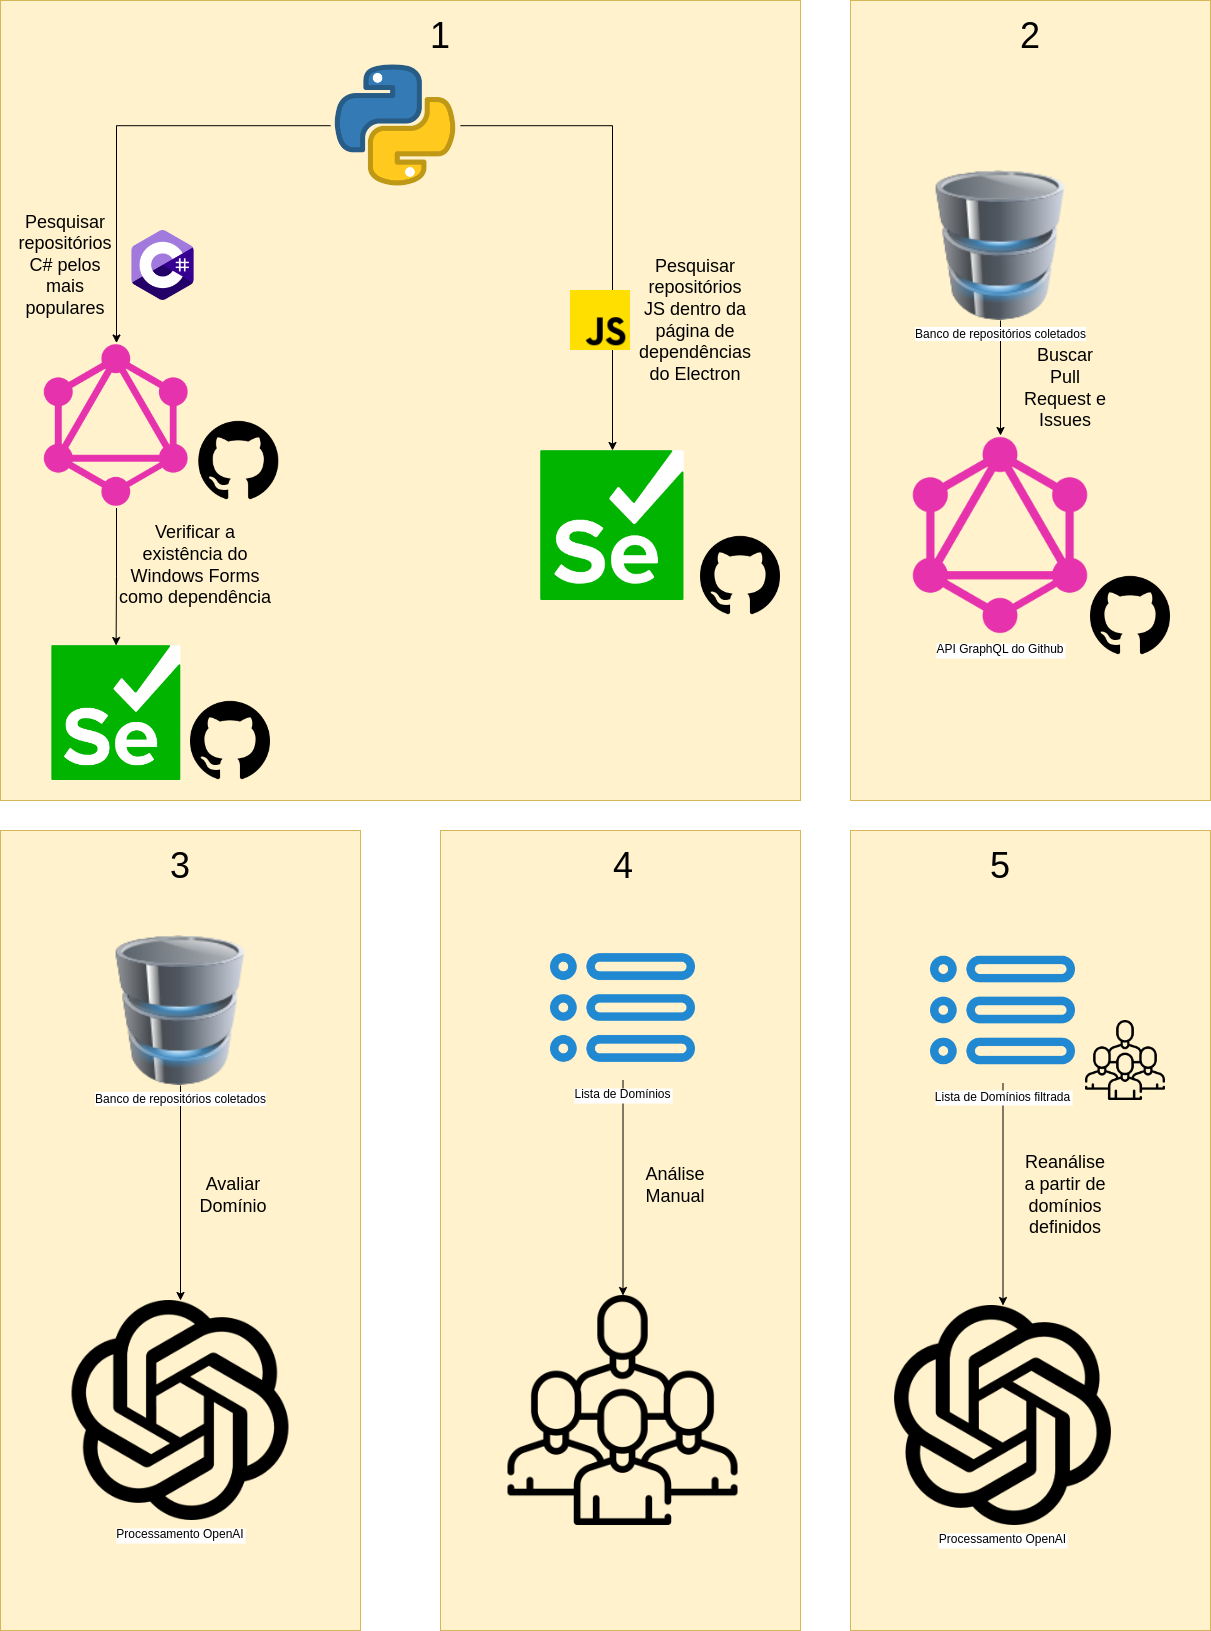
\includegraphics[width=0.6\textwidth]{images/metflow2.png}
    \caption{Metodologia}
    \label{fig:Metodologia}
\end{figure}

\subsection{Etapas da metodologia}

Nesta seção são apresentadas as cinco etapas utilizadas neste estudo exploratório de caracterização de domínios de aplicações desktops e suas popularidades.

\subsubsection{Coleta de repositórios}

Na Etapa 1, para realizar o filtro de quais repositórios estavam na categoria \textit{desktop} foram utilizados dois procedimentos, um para cada linguagem de programação. Além disso, para realizar a busca das dependências do projeto utilizou-se o Selenium, uma ferramenta de automação de testes para aplicações web, para auxiliar a realizar uma busca nos grafos de dependência dos repositórios, disponível na plataforma do Github, pois a API de GraphQL do Github não possui essa funcionalidade.

O primeiro procedimento, em C\# foi utilizado a API de GraphQL disponibilizada pela plataforma Github, através dessa interface, realizou-se uma busca ordenada pelos repositórios mais populares, conforme o número de estrelas~\cite{DBLP:journals/corr/abs-1811-07643}, os quais verificou-se que o software era construído utilizando Windows Forms (estrutura para criação de aplicativos da área de trabalho do Windows da linguagem C\#) através do grafo de dependência. O segundo procedimento, na linguagem Javascript, buscou todos os repositórios que utilizavam o Electron (framework para construir aplicações desktop usando Javascript, HTML e CSS), utilizando seu grafo de dependência.

\subsubsection{Recolhimento de \textit{issues} e \textit{pull requests}}

Sequencialmente, na Etapa 2, utilizando a lista de repositórios formada, foi coletado através da interface GraphQL do Github todos os \textit{pull requests} e \textit{issues} dos repositórios das duas linguagens recolhidos. O estudo considerou 1781 repositórios coletados no período de setembro a outubro de 2022, sendo 561 repositórios com mais de 300 estrelas em C\# e outros 1220 que possuem mais de 1000 estrelas feitos em Javascript

\subsubsection{Análise de Domínio Utilizando Inteligência Artificial}

A Etapa 3, no que lhe concerne, utilizou os repositórios obtidos na etapa anterior na plataforma de inteligência artificial denominada OpenAI, visando realizar a leitura de descrição de cada repositório e definir um domínio para ele, esse processo atribuiu 604 domínios únicos para os 1781 repositórios sendo que 395 repositórios foram descartados, porque a OpenAI não conseguiu identificar um domínio.

\subsubsection{Filtragem manual de domínios}

Posteriormente, na Etapa 4, a lista dos 604 domínios passou por uma análise manual feita pelos integrantes da pesquisa, para que domínios que possuírem semelhanças como: termos no plural e palavras semelhantes com apenas uma ocorrência fossem removidos e reavaliados novamente. Ao final da análise manual foram selecionados 68 domínios únicos, cujos foram utilizados para efetuar uma nova atribuição pela inteligência artificial.

\subsubsection{Reavaliação de repositórios com domínios definidos}

A Etapa 5 consistiu na OpenAI reavaliar os repositórios, utilizando os 68 domínios para decidir qual era o mais próximo da descrição, podendo também não definir nenhum caso julgasse muito fora do escopo do repositório ou caso não houvesse uma descrição definida.

\subsection{Hipóteses e Métricas}

Nesta seção será discorrido as questões de pesquisa, suas respectivas métricas e as hipóteses levantadas.

\subsubsection{QP.1}

Mediante ao cenário atual de popularização das tecnologias web, a decisão do tipo de plataforma em que um software deverá ser disponibilizado  deverá considerar uma série de fatores. Um deles fatores é se o domínio do software convém ser disponibilizado em plataforma \textit{desktop} atualmente. Sendo assim, foi levantada a seguinte questão: a QP.1 Para as aplicações \textit{desktop} que ainda são mantidas, qual o domínio que elas se encontram atualmente?

Para responder essa questão, foram definidas 2 métricas. A métrica M.1, sendo a proporção de repositórios que possuem descrições e domínios contra que não possuem descrições ou domínios visando exibir a quantidade de repositórios \textit{desktops} que declararam sobre o que se trata seu software. A métrica M.2 sendo o percentual da quantidade de repositórios \textit{desktops} para cada domínio a fim de identificar os principais domínios cujas aplicações \textit{desktops} ainda são utilizadas e consequentemente haverá sentido disponibilizar uma versão desktop de uma aplicação dentro desses domínios. A hipótese inicial tem-se de que os principais domínios seriam voltados para aplicações de antivírus, editores de imagens e vídeos, compartilhamento de tela, pois essas aplicações exigem maior contato com os recursos do hardware, levando vantagem em ser utilizadas via \textit{desktop}.

\subsubsection{QP.2}

Um fator que é de suma importância para manutenção do software é saber se a tecnologia escolhida terá longevidade, ao passo que escolher uma tecnologia aonde a tendência é a depreciação resultará em dificuldades ao resolver problemas e obter mão de obra para tal. Dado este fato, foi levantada a nossa segunda questão: a QP.2 A quantidade de aplicações \textit{desktop} vem diminuindo ao longo da última década?

Para responder essa questão, foram definidas 2 métricas. A métrica M.3, sendo a média de repositórios com dependências de aplicações\textit{desktop} criados por ano para cada domínio. A M.4, é a média de repositórios com dependências de aplicações \textit{desktop} por ano, independente do domínio. O objetivo dessas métricas é exibir a tendência de repositórios \textit{desktops} dos últimos anos para cá, seja por um domínio específico ou não. Dado a popularização e o crescimento de tecnologias web, é provável que há uma tendência de queda para os repositórios \textit{desktops} de 2018 até a atualidade.

\subsubsection{QP.3}

A comunidade de uma tecnologia é outro fator importante para definir a arquitetura do software, pois ao surgirem dúvidas ou problemas durante o desenvolvimento de um software é de suma importância que existam usuários engajados na comunidade que passaram por algo semelhante e podem ajudar a lidar com esse problema~\cite{9282287}. Isto posto, foi levantada a seguinte questão: a QP.3 Aplicações desktop tem engajamento da comunidade? 
 
Para responder essa questão, foram definidas 2 métricas. A métrica M.5, sendo percentual de \textit{pull requests merged} relação aos que não foram \textit{merged} por ano, para ilustrar cronologicamente a contribuição da comunidade quanto a softwares \textit{desktops}. Dado a popularização e o crescimento de tecnologias web, é provável que há uma tendência de queda para os \textit{pull requests} de repositórios \textit{desktop} de 2018 até a atualidade. A métrica M.6, definida como a exibição do percentual de \textit{issues} fechadas em relação a não fechadas em repositórios \textit{desktops} por ano, com o propósito de mostrar se os problemas relatados vêm sendo resolvidos durante os anos. Dado a popularização e o crescimento de tecnologias web, possivelmente há uma queda na quantidade de \textit{issues} de repositórios desktops de 2018 até a atualidade.

\subsection{Análise de resultado} 

Os dados coletados na etapa de mineração passaram por tratamentos via MySQL que possibilitou a extração das quantidades de repositórios agrupados por domínio, \textit{issues}, \textit{pull requests} e os anos. Em seguida os dados foram exportados para planilhas do \emph{Google Sheets} aonde foi feita a adequação dos dados para a importação da planilha no \emph{Google DataStudio}, ferramenta do Google que foi utilizada para a geração dos relatórios e painéis informativos que possibilitaram uma análise visual dos resultados descritos na seção abaixo.

\section{Resultados} \label{resultados}

Após realização de todo processo descrito na metodologia e análise dos dados coletados, os seguintes resultados para responder às questões de pesquisa (QP.1, QP.2 e QP.3) foram encontrados conforme as métricas definidas (M.1, M.2, M.3, M.4, M.5e e M.6) e calculadas com os dados buscados. Os gráficos apresentados nessa seção foram criados na ferramenta \emph{Google DataStudio}.

\subsection{Métricas da QP.1}

Em vista da métrica M.1, referente a QP.1, que consiste na proporção entre repositórios de aplicações desktop que possuem descrições e domínios e os que não possuem, foram encontrados os dados descritos na Tabela \ref{tab:descricao x sem descricao}{}.
\begin{table}[H]
    \caption{Repositórios de aplicações desktop com e sem domínio definido X Quantidade de repositórios desktops}
    \centering
    \label{tab:descricao x sem descricao}
        \begin{tabular}{|l|l|l|}
        \hline
        Repositório & Quantidade & Percentual\\
        \hline
        Sem domínio ou sem descrição & 395 & 22.17\%\\
        \hline
        Com domínio & 1386 & 77.83\%\\
        \hline
        \end{tabular}
\end{table}
Dos 1781 repositórios coletados durante o tempo hábil dessa pesquisa, foi possível definir domínios, por meio da ferramenta OpenAI, os repositórios que possuem descrição e domínio (77.83\%) e os que não possuem (22.17\%). Os repositórios que não tiveram as descrições encontradas foram os que não possuíam o campo \emph{description} em suas páginas do Github e também outros que a inteligência artificial não obteve sucesso ao tentar encontrar um domínio pela \emph{description}, sendo válido considerar que após os resultados da OpenIA, foi feita uma tentativa de classificar tais repositórios sem domínios manualmente, contudo foi inválida, por falta de informações nos repositórios. 

Para a métrica M.2, da QP.1, o percentual de repositórios de aplicações desktop para cada domínio, foram obtidos os resultados descritos na Figura \ref{fig:Percentual de repositórios por domínio}.
\begin{figure}[H]
    \centering
    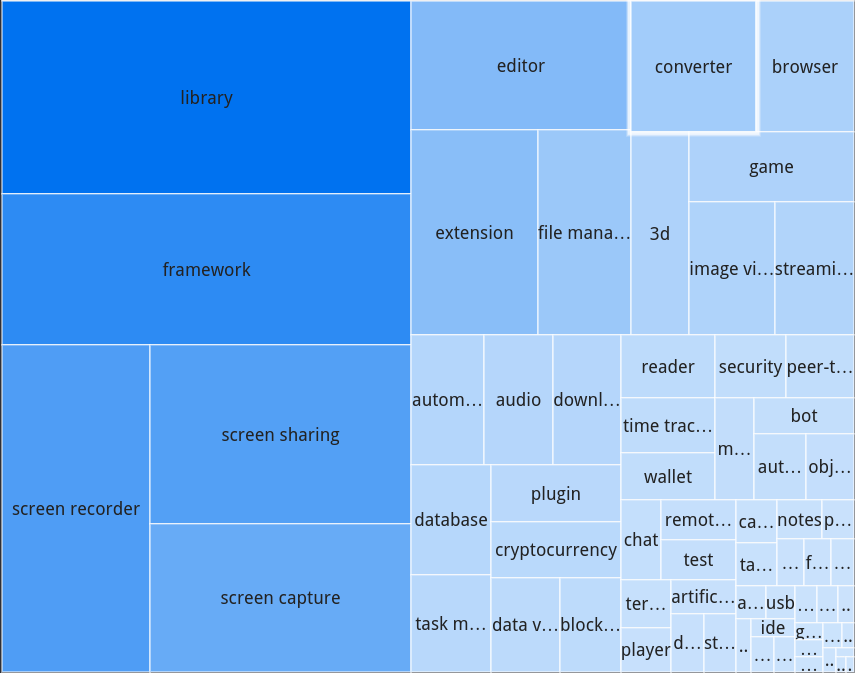
\includegraphics[width=0.9\textwidth]{images/dominios map.png}
    \caption{Percentual de repositórios de aplicações desktop para cada domínio}
    \label{fig:Percentual de repositórios por domínio}
\end{figure}
Dessa forma, com as métricas encontradas, é possível ver maior dominância dos domínios: \emph{Library} (Bibliotecas), \emph{Frameworks}, \emph{Screen Sharing}(Compartilhamento de tela), \emph{Screen recorder}(Gravador de tela), \emph{Screen capture}(Capturador de tela), \emph{Editor de texto}, \emph{Extension}(Extensões), \emph{File Management}(Gerenciador de Arquivos), \emph{Conversor}(Conversores), \emph{Browser}(Navegador).

\subsection{Métricas da QP.2}

Para a métrica M.1, da QP.2, que consiste na média de repositórios de aplicações \emph{desktop} criados por ano para cada domínio, os resultados obtidos estão representados na Figura \ref{fig:10 domínios mais frequentes}, onde para efeito de melhor observabilidade foram selecionados apenas os 10 domínios mais frequentes no gráfico.
\begin{figure}[H]
    \centering
    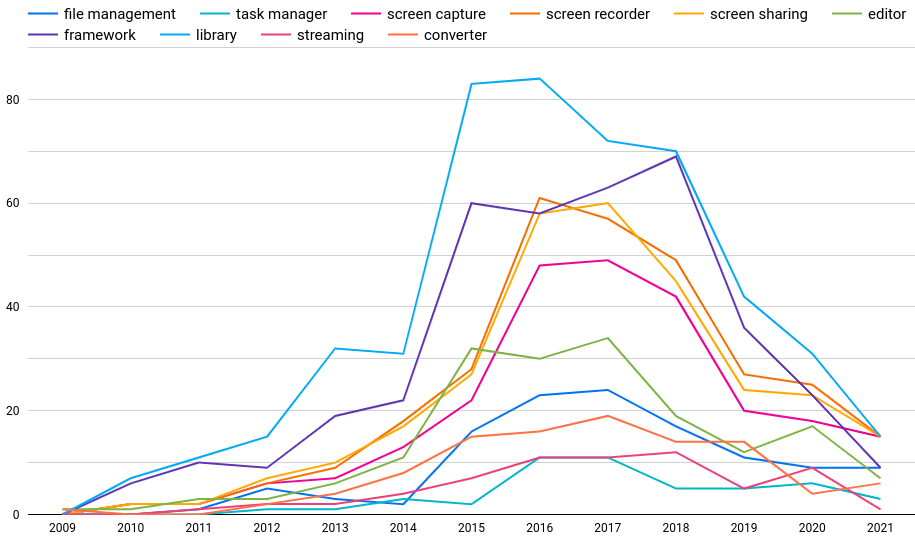
\includegraphics[width=0.9\textwidth]{images/10 dom mais fre.png}
    \caption{10 domínios mais frequentes}
    \label{fig:10 domínios mais frequentes}
\end{figure}
É possível observar na Figura \ref{fig:10 domínios mais frequentes} que houve um momento de pico na criação de repositórios de aplicações desktop no ano de 2016, seguido por uma queda até a metade do ano de 2022 (ano em que a pesquisa foi realizada). 

Para a métrica M.2, da QP.2, que consiste na média de repositórios com dependências de aplicações desktops criados por ano, foram encontrados os resultados apresentados na Figura \ref{fig:Repositório de aplicações desktop criados de cada linguagem criados por ano}.
\begin{figure}[H]
    \centering
    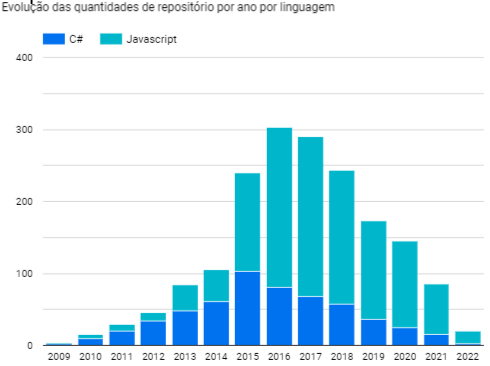
\includegraphics[]{images/lang por ano.png}
    \caption{Repositório de aplicações desktops criados de cada linguagem criados para cada ano}
    \label{fig:Repositório de aplicações desktop criados de cada linguagem criados por ano}
\end{figure}
Na Figura \ref{fig:Repositório de aplicações desktop criados de cada linguagem criados por ano} a evolução segue a mesma tendência da Figura \ref{fig:10 domínios mais frequentes}, pois estão diretamente relacionadas. Os repositórios da linguagem Javascript possuem maiores quantidades, pois representam a maioria dos repositórios coletados na pesquisa.

\subsection{Métricas da QP.3}

Para a métrica M.1, da QP.3, que consiste no percentual de \emph{pull Requests merged} e \emph{pull requests not merged}, os resultados obtidos são apresentados na Figura \ref{fig:Evolução dos Pull Requests por ano}. É possível observar o crescimento tanto dos \emph{pull requests merged} quanto dos  \emph{pull requests not merged}
\begin{figure}[H]
    \centering
    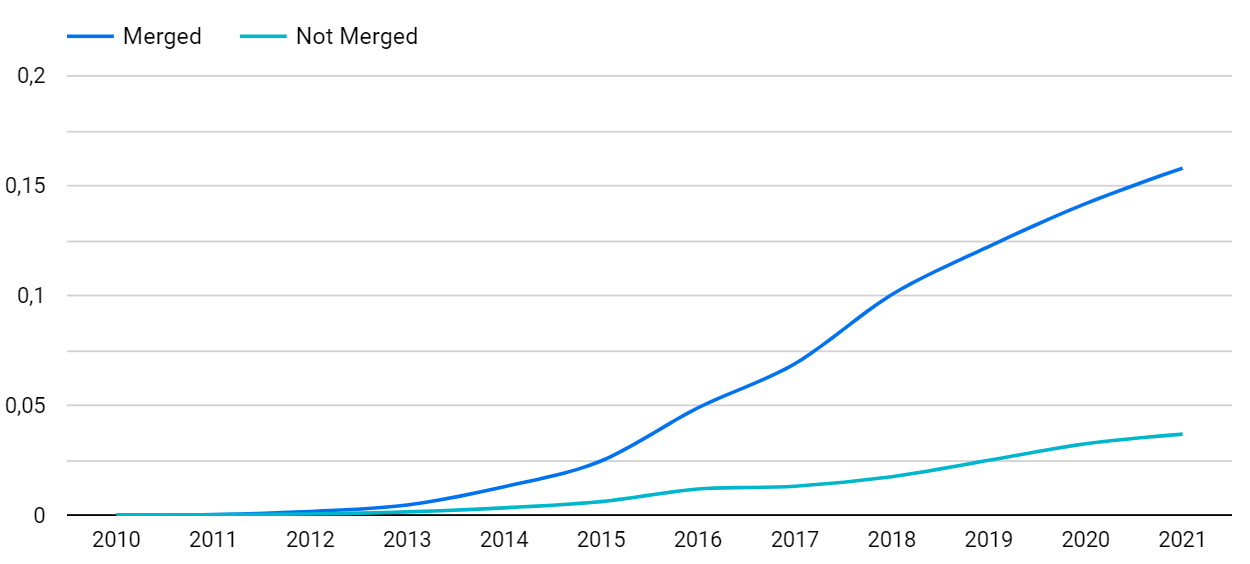
\includegraphics[width=0.9\textwidth]{images/percentual por ano PR.png}
    \caption{Evolução dos \emph{pull requests} por ano}
    \label{fig:Evolução dos Pull Requests por ano}
\end{figure}

Para a métrica M.2, da QP.3, o percentual de \emph{issues} fechadas e  \emph{issues} abertas, os resultados se encontram na Figura \ref{fig:Evolução das Issues por ano}.
\begin{figure}[H]
    \centering
    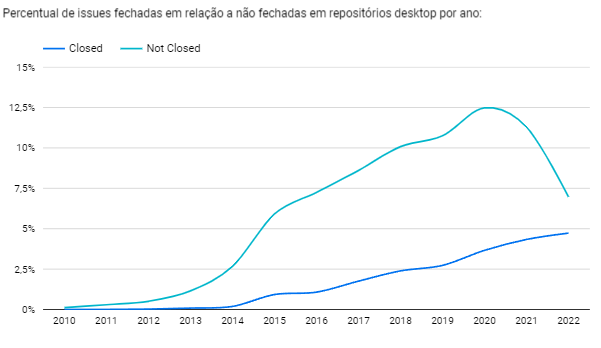
\includegraphics[width=0.9\textwidth]{images/issues por ano.png}
    \caption{Evolução das \emph{issues} por ano}
    \label{fig:Evolução das Issues por ano}
\end{figure}
Na Figura \ref{fig:Evolução das Issues por ano} nota-se que desde o começo da coleta, no ano de 2010, até o ano de 2020 as \emph{issues} fechadas cresceram em quantidade. Entretanto, após 2020, caíram. Já as \emph{issues} abertas, apresentaram crescimento em todo o percurso analisado. Sendo assim, é possível ver que existe um engajamento da comunidade considerando a diminuição de \emph{issues} abertas e \emph{pull requests merged}.

\bibliographystyle{sbc}
\bibliography{sbc-template}

\end{document}
